\section{Curved Lines}

An equation involving $x$ and $y$ gives a \term{curve}\index{Curved Line} in the plane.

By replacing $x$ with $x - a$, the graph is shifted to the right by $a$. By replacing $y$ with $y - b$, the graph is shifted upward by $b$.

\begin{center}
    \tikzsetnextfilename{c01s01-f01}%
    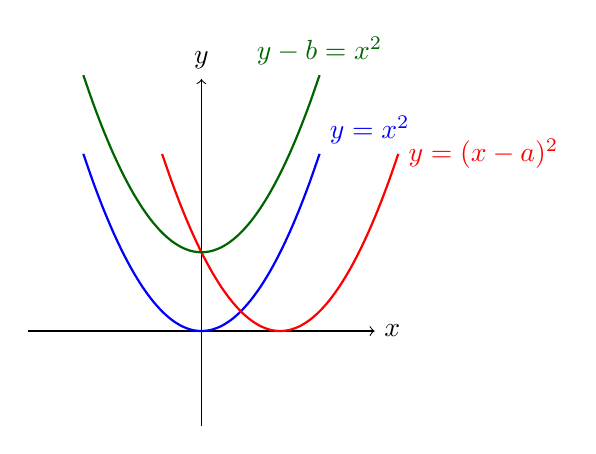
\begin{tikzpicture}
        \draw[->] (-2.2, 0) -- (2.2, 0) node[right] {$x$};
        \draw[->] (0, -1.2) -- (0, 3.2) node[above] {$y$};

        \draw[thick,blue,domain=-1.5:1.5,smooth] plot (\x,{(\x)^2}) node [above right] {$y = x^2$};
        \draw[thick,red,domain=-0.5:2.5,smooth] plot (\x,{(\x - 1)^2}) node [right] {$y = (x - a)^2$};
        \draw[thick,DarkGreen,domain=-1.5:1.5,smooth] plot (\x,{(\x)^2 + 1}) node [above] {$y - b = x^2$};
    \end{tikzpicture}
\end{center}

\begin{definition}[Parabola]\index{Parabola}
    The \term{parabola} (with vertex) at the origin is defined by $$y = ax^2 \qquad x = by^2$$

    \begin{itemize}
        \item $y = ax^2$ opens up for $a > 0$, and opens down for $a < 0$.
        \item $x = by^2$ opens to the right for $b > 0$, and opens to the left for $b < 0$.
    \end{itemize}
\end{definition}

\begin{center}
    \tikzsetnextfilename{c01s01-f02}%
    \begin{tikzpicture}
        \draw[->] (-2.2, 0) -- (2.2, 0) node[right] {$x$};
        \draw[->] (0, -1.2) -- (0, 3.2) node[above] {$y$};

        \draw[thick,blue,domain=-1.5:1.5,smooth] plot (\x, {(\x)^2}) node [above] {$y = ax^2$};
    \end{tikzpicture}
    \qquad
    \tikzsetnextfilename{c01s01-f03}%
    \begin{tikzpicture}
        \draw[->] (-1.2, 0) -- (3.2, 0) node[right] {$x$};
        \draw[->] (0, -2.2) -- (0, 2.2) node[above] {$y$};

        \draw[thick,blue,domain=0:2.5,smooth] plot (\x, {sqrt(\x)}) node [above] {$x = by^2$};
        \draw[thick,blue,domain=0:2.5,smooth] plot (\x, {-sqrt(\x)});
    \end{tikzpicture}
\end{center}

\begin{definition}[Ellipse]\index{Ellipse}
    The \term{ellipse} (with center) at the origin is defined by $$\left(\frac{x}{a}\right)^2 + \left(\frac{y}{b}\right)^2 = 1$$ with $(a, 0)$ being the right-most point on the $x$-axis, and $(0, b)$ as the top-most point on the $y$-axis.

    When $a = b$, an ellipse becomes a \term{circle}, with $a = b = R$ as the radius of the circle \footnote{$\left(\frac{x}{R}\right)^2 + \left(\frac{y}{R}\right)^2 = 1 \implies x^2 + y^2 = R^2$}.
\end{definition}

\begin{center}
    \tikzsetnextfilename{c01s01-f04}%
    \begin{tikzpicture}
        \draw[->] (-3.2, 0) -- (3.2, 0) node[right] {$x$};
        \draw[->] (0, -1.7) -- (0, 1.7) node[above] {$y$};

        \draw[thick,blue] (0, 0) ellipse (2cm and 1cm);

        \draw[thick,red] (2, 0.25) -- (2, 0) node[below,red] {$a$};
        \draw[thick,red] (0.25, 1) -- (0, 1) node[left,red] {$b$};
    \end{tikzpicture}
\end{center}

\begin{definition}[Hyperbola]\index{Hyperbola}
    The \term{hyperbola} (with center) at the origin is defined by $$\left(\frac{x}{a}\right)^2 - \left(\frac{y}{b}\right)^2 = 1 \qquad \left(\frac{y}{a}\right)^2 - \left(\frac{x}{b}\right)^2 = 1$$

    A hyperbola has 2 curves, and a center line that is not crossed. The 2 curves goes in the opposite direction of the center.
\end{definition}

\begin{center}
    \tikzsetnextfilename{c01s01-f05}%
    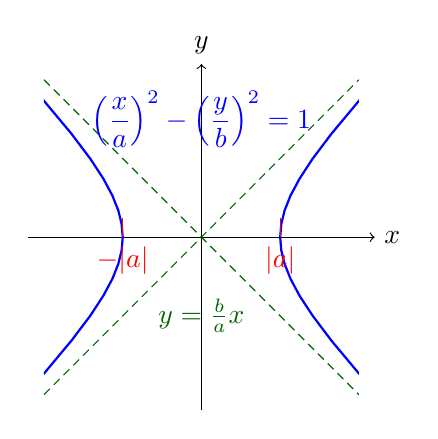
\begin{tikzpicture}
        \draw[->] (-2.2, 0) -- (2.2, 0) node[right] {$x$};
        \draw[->] (0, -2.2) -- (0, 2.2) node[above] {$y$};

        \clip(-2, -2) rectangle (2, 2);

        \draw[thick,blue,domain=-0.99:0.99] plot ({( 1+(\x)^2)/(1-(\x)^2)}, {  2 *(\x)/(1-(\x)^2)});
        \draw[thick,blue,domain=-0.99:0.99] plot ({(-1-(\x)^2)/(1-(\x)^2)}, {(-2)*(\x)/(1-(\x)^2)});

        \draw[densely dashed,DarkGreen,domain=-2:2] plot (\x, \x);
        \draw[densely dashed,DarkGreen,domain=-2:2] plot (\x, -\x);
        \node[DarkGreen] at (0,-1) {$y = \frac{b}{a}x$};

        \draw[red] (-1,0.25) -- (-1,0) node[below] {$-|a|$};
        \draw[red] (1,0.25) -- (1,0) node[below] {$|a|$};
        \node[blue] at (0,1.5) {$\displaystyle \left(\frac{x}{a}\right)^2 - \left(\frac{y}{b}\right)^2 = 1$};
    \end{tikzpicture}
\end{center}

Since the right side is positive, and a square is positive, the position of the negative sign determines the direction of the curves.

To determine the direction, we can either set $x = 0$ or $y = 0$. For example, in the case of $x^2 - y^2 = 1$, by setting $x = 0$, we attain $-y^2 = 1$ is impossible, so the vertical line $x = 0$ is the center is never crossed. Thus the 2 curves open towards left and right.

To find the \bred{slant asymptotes} when $x$ and $y$ are both large, change the number $1$ on the right side of the equation to $0$.

{~~~}

The above 3 curves together are sometimes called: \term{Conic Sections}\index{Conic Sections}.

\section{Curved Surfaces}

An equation involving $x$, $y$, and $z$ gives a \term{curved surface}\index{Curved surface} in 3D space. In general, this surface is difficult to imagine and sketch in 3D.

\begin{definition}[3D Sphere]\index{Sphere}
    The \term{3D Sphere} (with center) at the origin with radius $R$ is given by $$x^2 + y^2 + z^2 = R^2$$
\end{definition}

\begin{center} 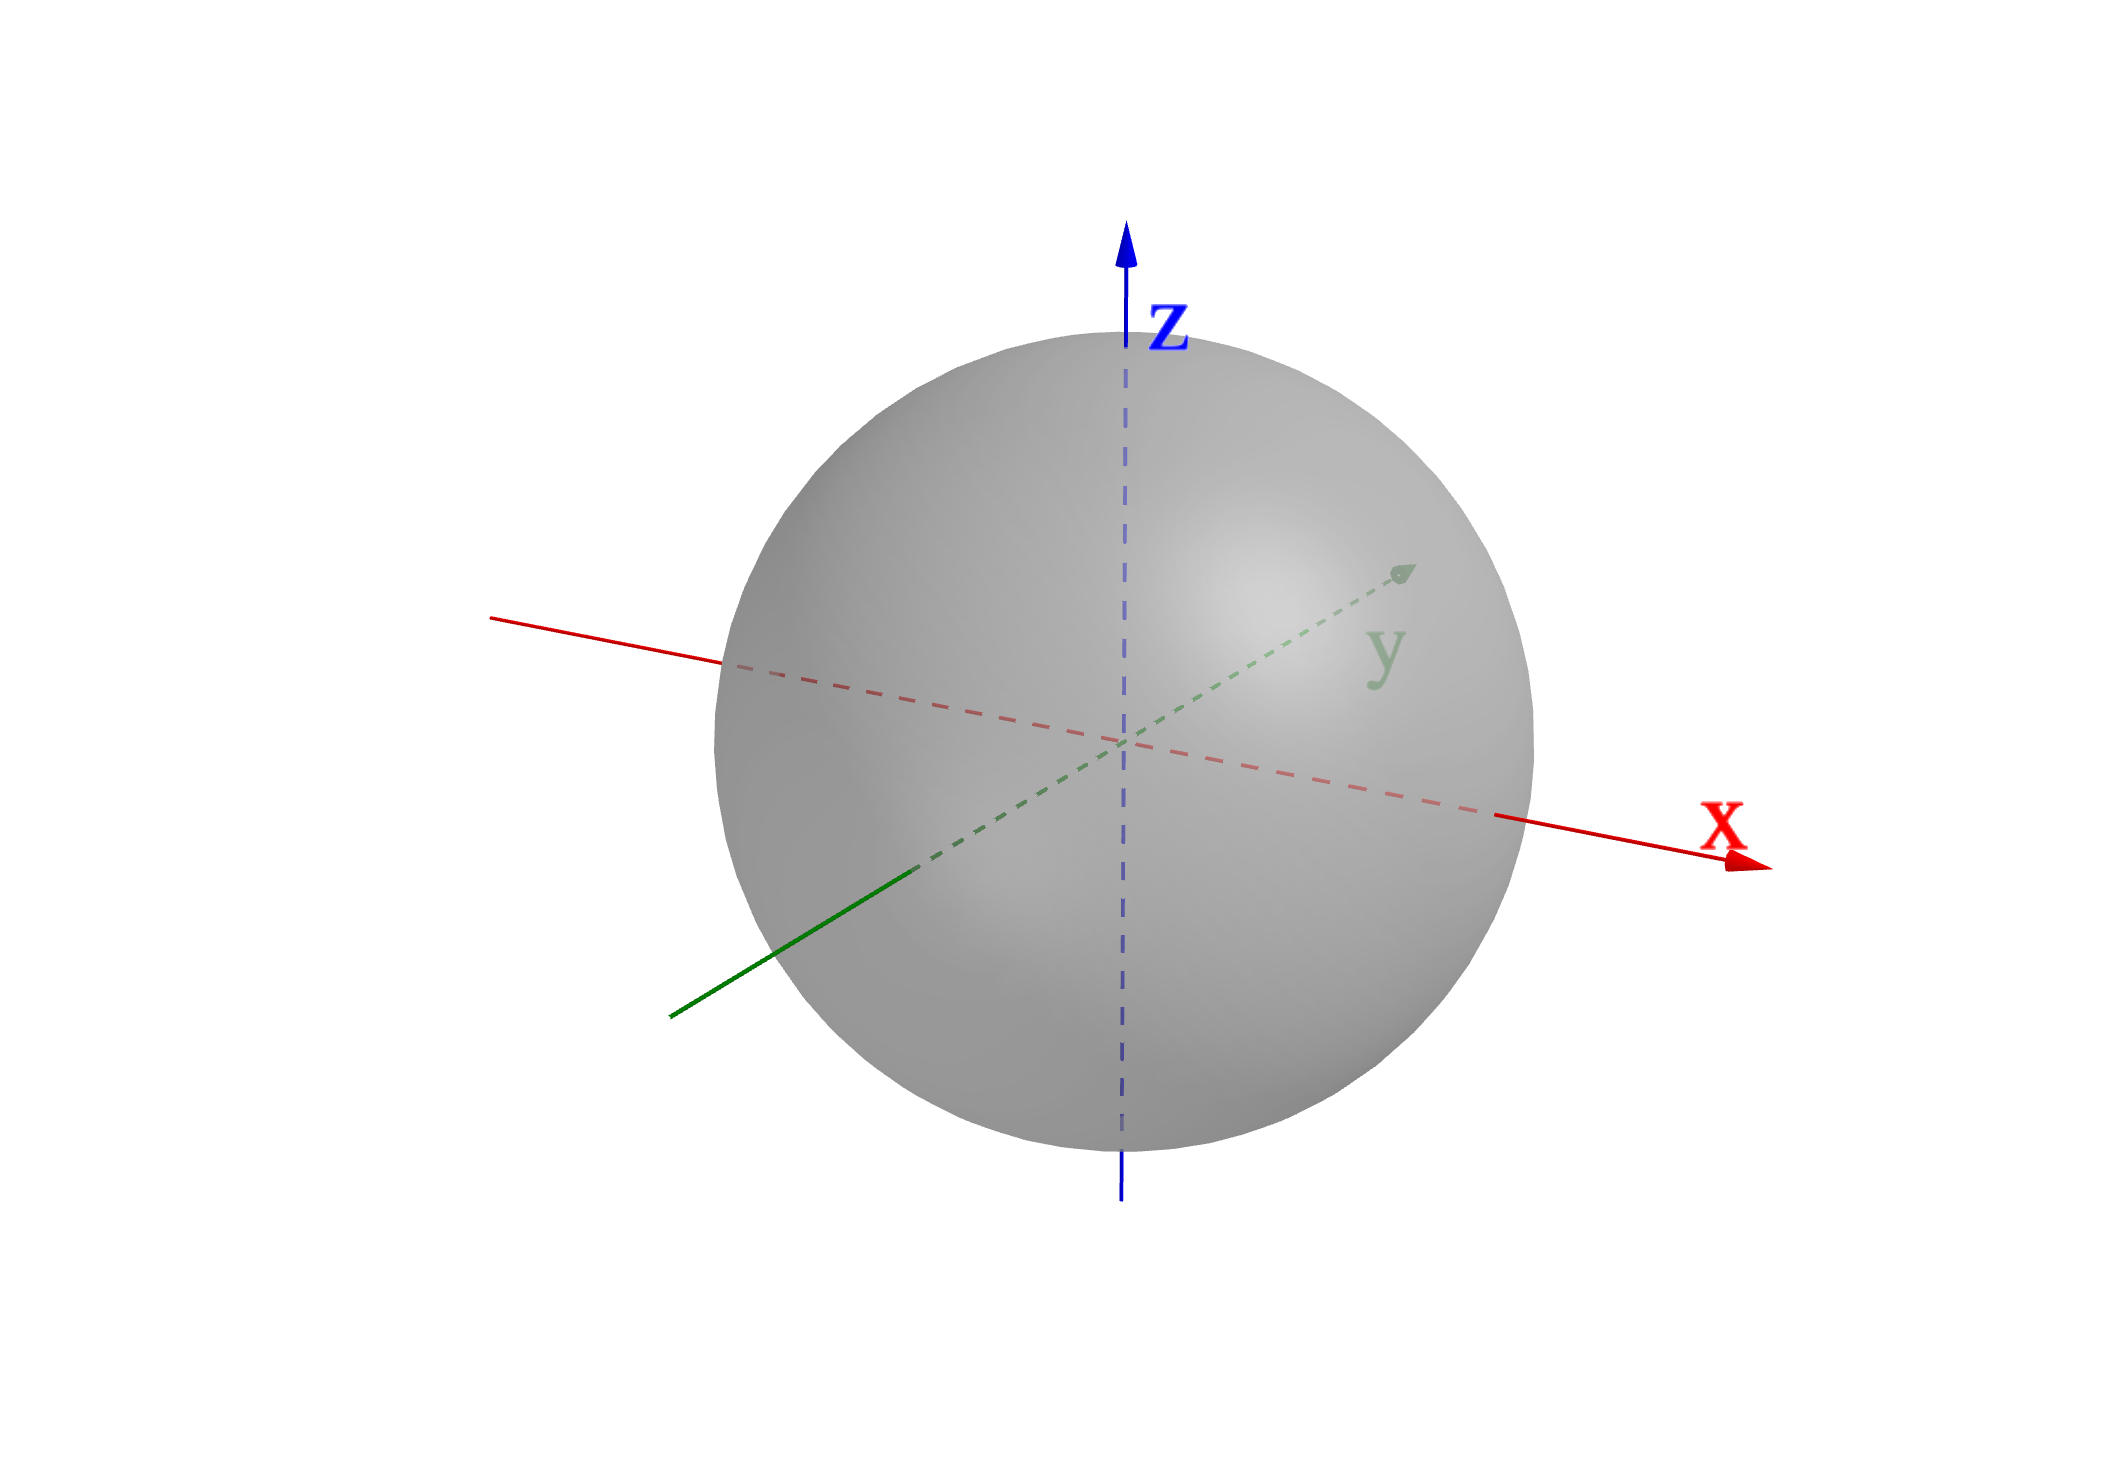
\includegraphics[width=0.5\textwidth]{Plots/sphere.png} \end{center}

\begin{definition}[Ellipsoid]\index{Ellipsoid}
    The 3D \term{ellipsoid} (with center) at the origin is given by $$\left(\frac{x}{a}\right)^2 + \left(\frac{y}{b}\right)^2 + \left(\frac{z}{c}\right)^2 = 1$$

    $(a, 0, 0)$, $(0, b, 0)$, $(0, 0, c)$ are the 3 points on the ellipsoid, similar to the ellipse.

    When $a = b = c$, an ellipsoid becomes a \term{sphere}, with $a = b = c = R$ as the radius.
\end{definition}

\begin{center} 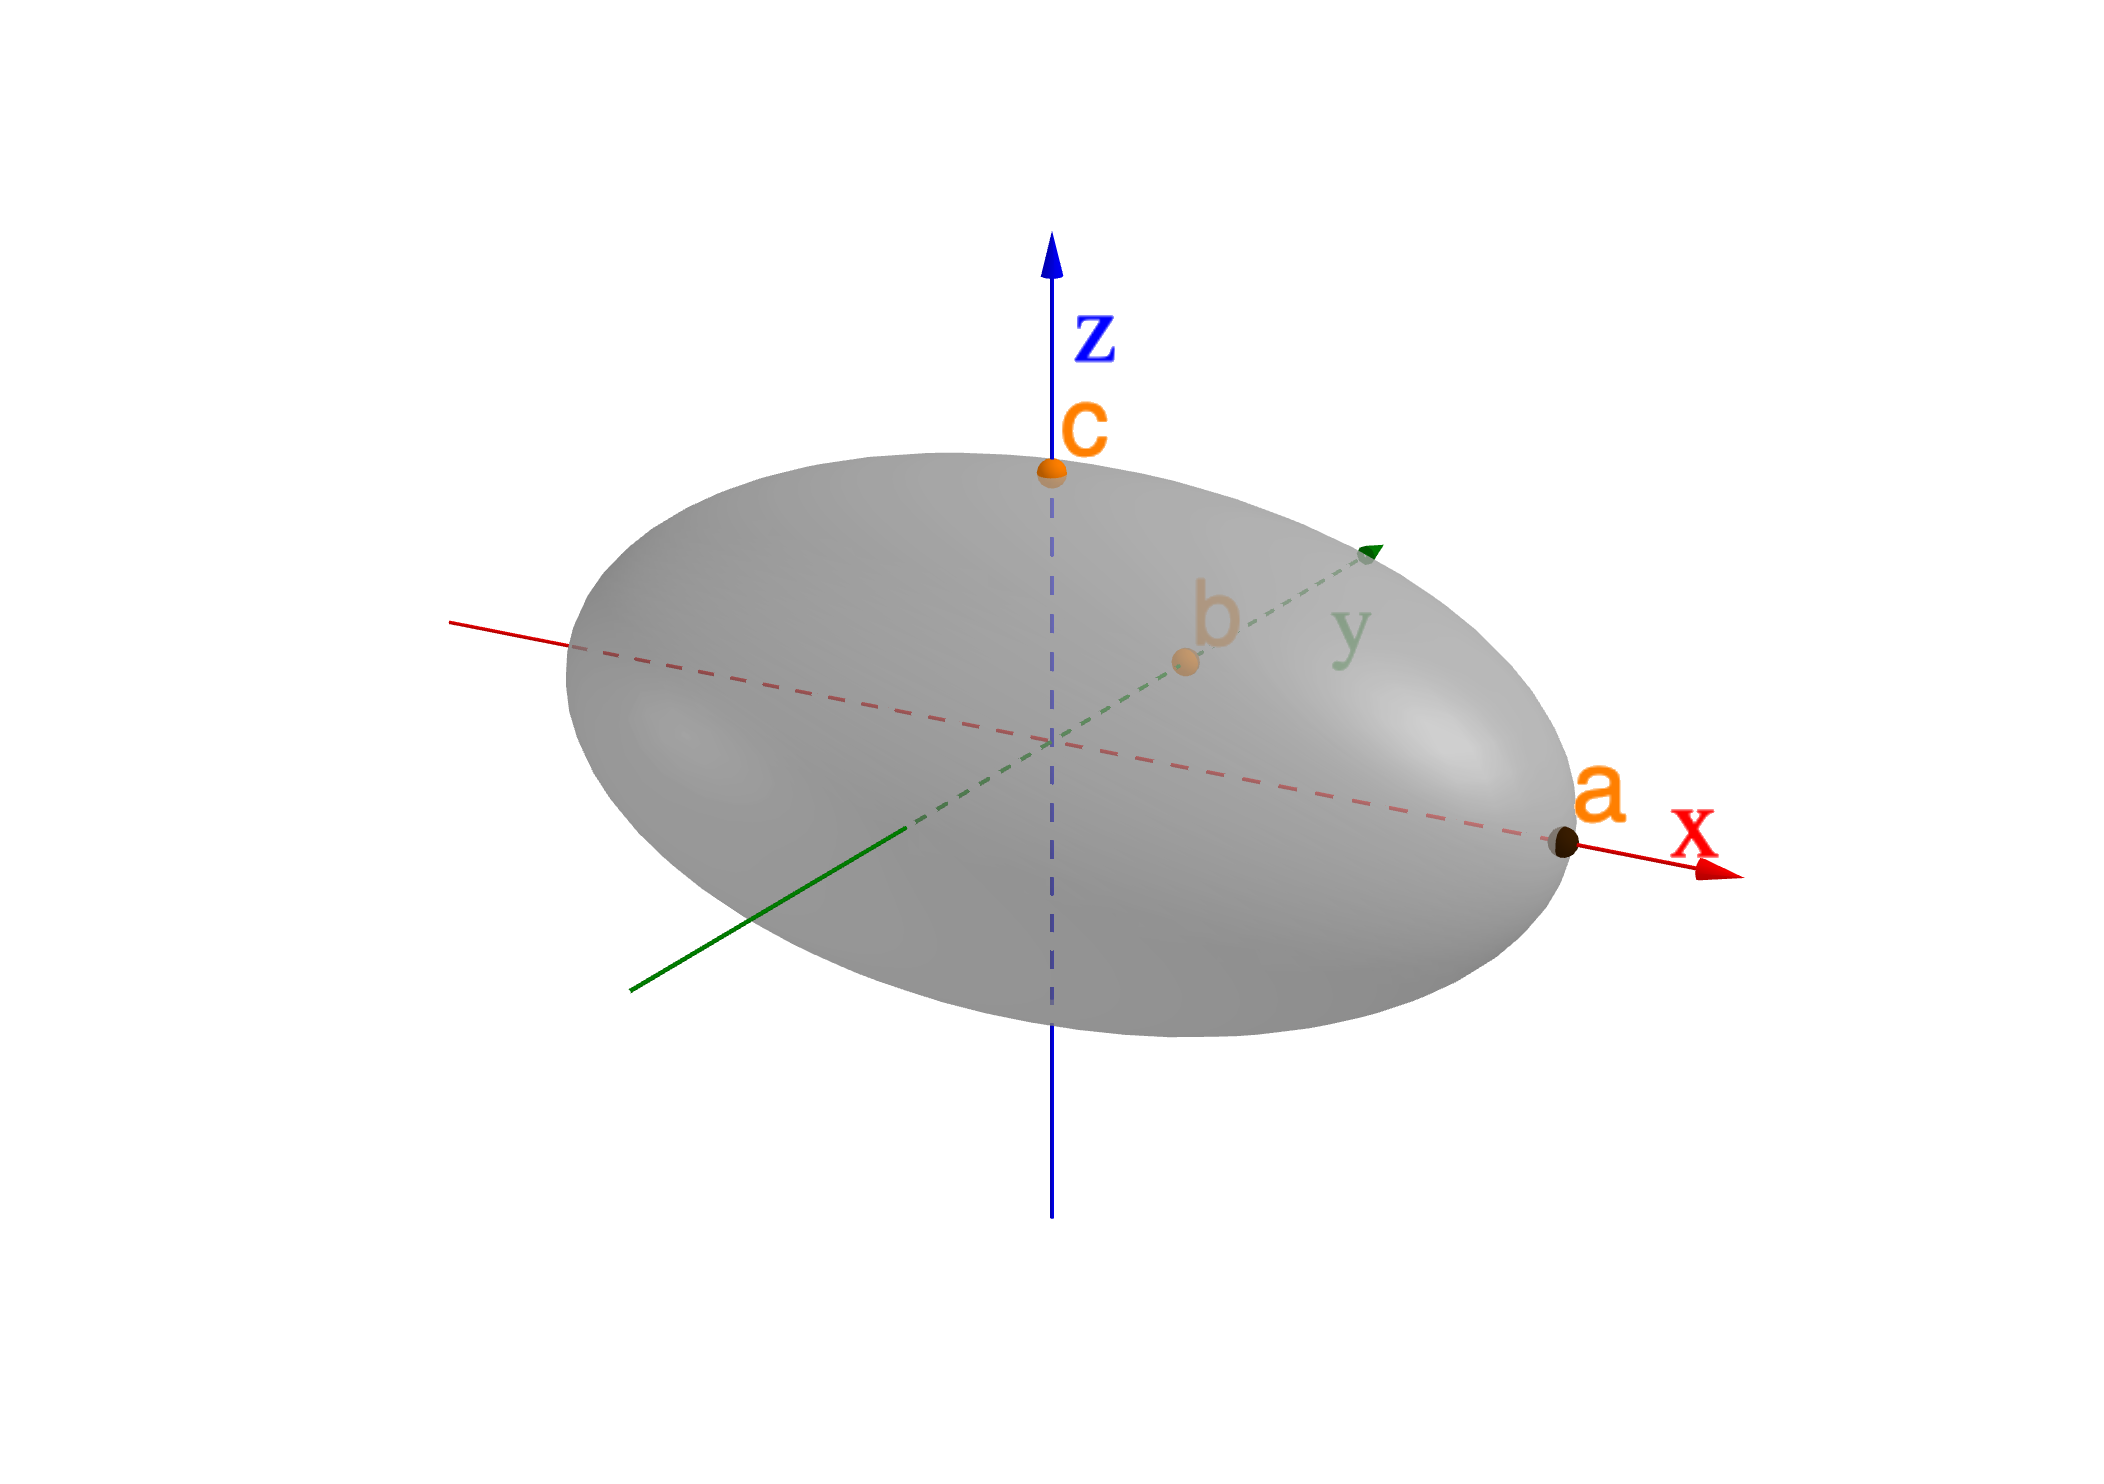
\includegraphics[width=0.5\textwidth]{Plots/ellipsoid.png} \end{center}

\subsubsection*{Surfaces Attained Through Rotation: $r^2 = x^2 + y^2$}

When the variables $x$ and $y$ appear together as $x^2 + y^2$, this signals that the surface is attained through rotation. Set a new variable $r$, with $r^2 = x^2 + y^2$. We graph the equation involving $z$ and $r$ in the $rz$-plane, with $r > 0$ only. We then revolve the curve around the $z$-axis to attain the surface in 3D: the $r$-axis stands for both $x$-axis and $y$-axis.

\begin{exercise}
    Sketch the following curves.

    \begin{minipage}[t]{0.45\linewidth} \setstretch{2.25}
        \begin{enumerate}
            \item $x = 2y^2$
            \item $\frac{x^2}{2} + \frac{y^2}{9} = 1$
            \item $x^2 + 2y^2 = 4$
        \end{enumerate}
    \end{minipage}
    \begin{minipage}[t]{0.45\linewidth} \setstretch{2.25}
        \begin{enumerate} \setcounter{enumi}{3}
            \item $x^2 + 3y^2 + 2x - 12y + 10 = 0$
            \item $y^2 - x^2 = 1$
            \item $\frac{(x - 2)^2}{4} - \frac{(y + 2)^2}{9} = 1$
        \end{enumerate}
    \end{minipage}
\end{exercise}

\begin{exercise}
    Sketch the following surfaces.

    \begin{minipage}[t]{0.45\linewidth} \setstretch{2.25}
        \begin{enumerate}
            \item $x^2 + y^2 = 1$

            \item $z = x^2 + y^2$

            \item $z^2 = x^2 + y^2$
        \end{enumerate}
    \end{minipage}
    \begin{minipage}[t]{0.45\linewidth} \setstretch{2.25}
        \begin{enumerate} \setcounter{enumi}{3}
            \item $x^2 + y^2 + \frac{z^2}{4} = 1$
            \item $z = \left( \sqrt{x^2 + y^2} - 1 \right)^2$
            \item $x^2 + y^2 + z^2 = 2z$
        \end{enumerate}
    \end{minipage}
\end{exercise}